\documentclass{article}

\usepackage{graphicx}
\usepackage{tikz}
\usepackage{tikzsymbols}
\usetikzlibrary{calc,patterns,shapes.geometric}
\pagestyle{empty}
\usepackage[margin=0pt]{geometry}
\geometry{papersize={14in,12in}}

\def\centerarc[#1](#2)(#3:#4:#5){\draw[#1] ($(#2)+({#5*cos(#3)},{#5*sin(#3)})$) arc (#3:#4:#5);}

\begin{document}
	\begin{figure}
		\centering
		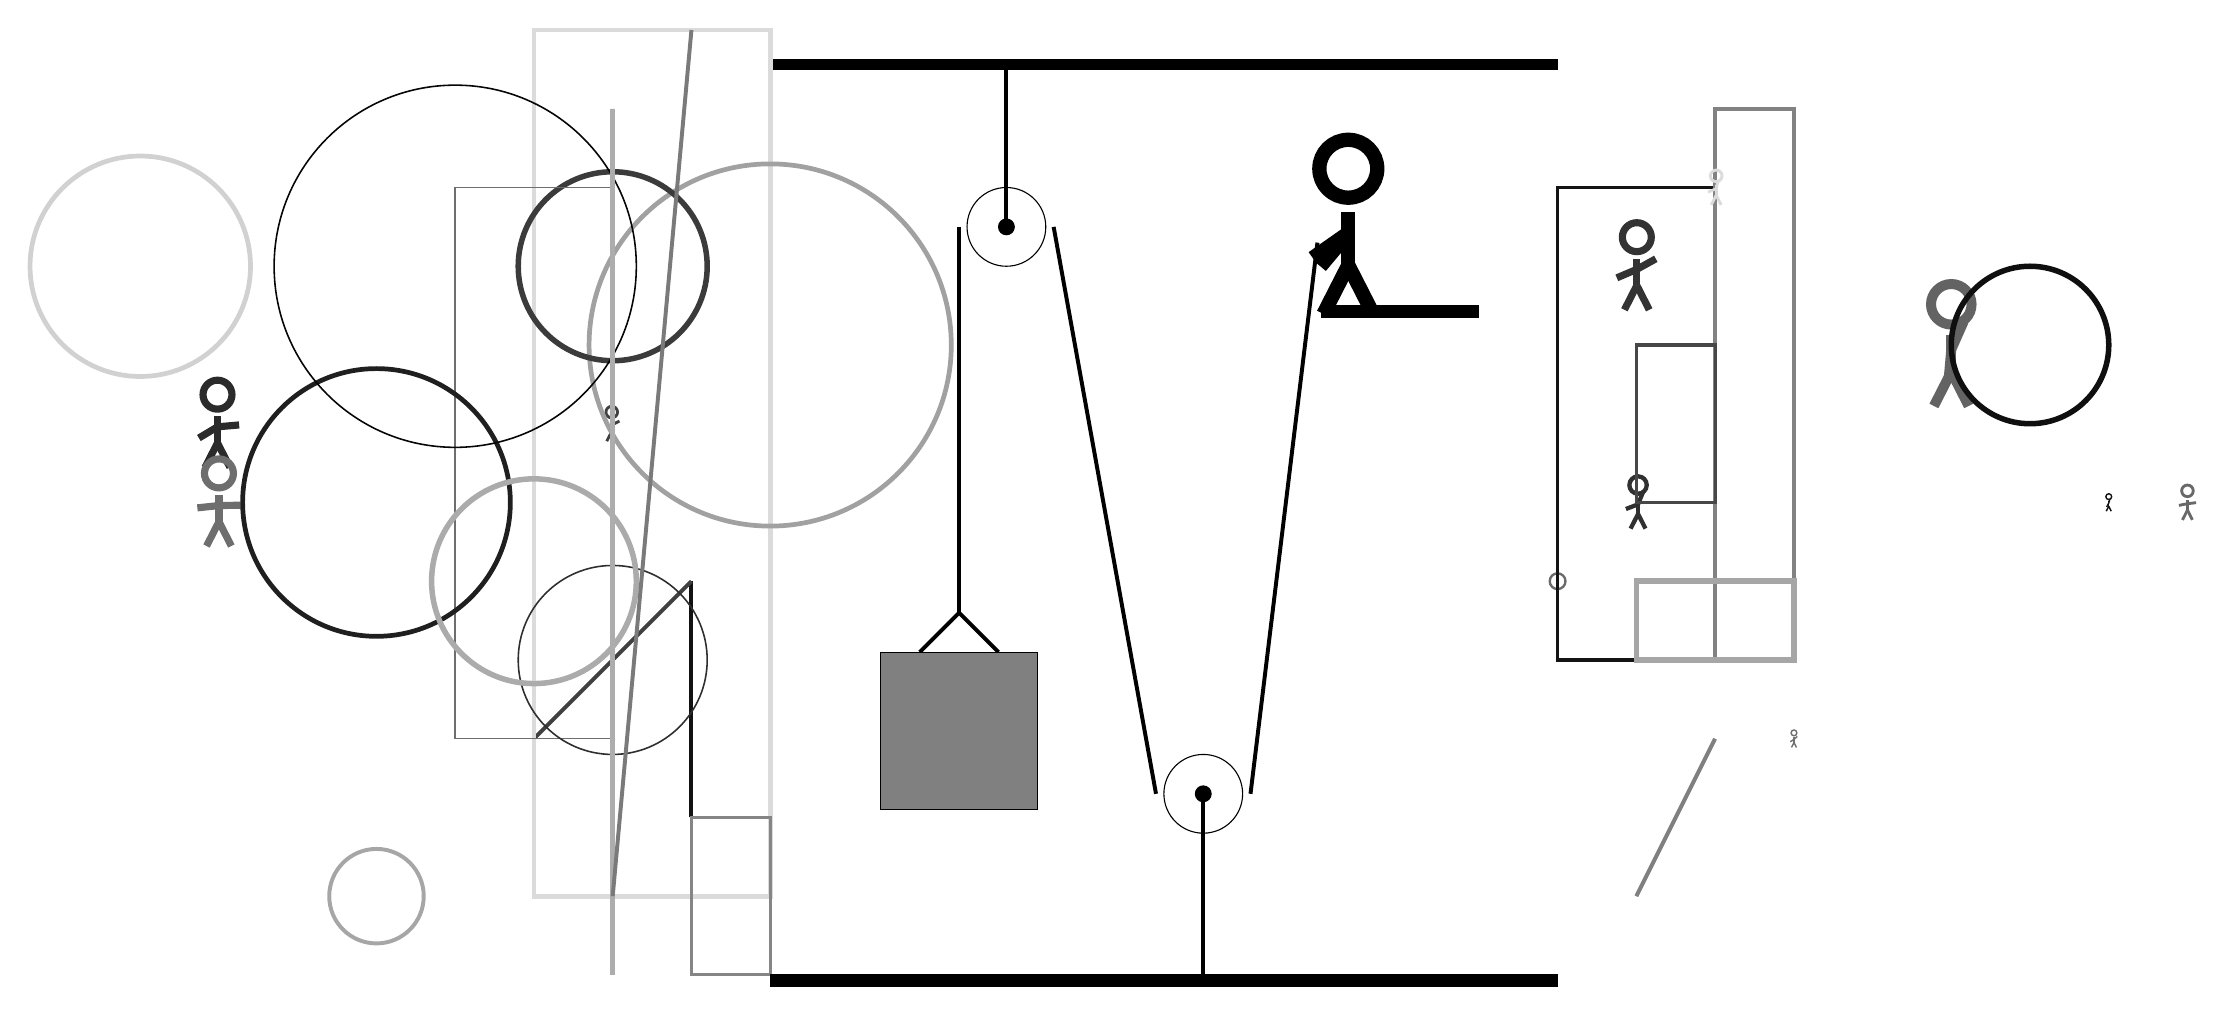
\begin{tikzpicture}
			%%%%% START %%%%%
			
			\draw[fill=black] (-2, 11.5) rectangle (8, 11.625);
			
			\draw (3.5, 2.3) circle (0.5);
			\draw[fill=black] (3.5, 2.3) circle (0.1);
			\draw[line width=0.5mm] (3.5, 2.3) -- (3.5, 0);
			
			\draw (1, 9.5) circle (0.5);
			\draw[fill=black] (1, 9.5) circle (0.1);
			\draw[line width=0.5mm] (1, 11.5) -- (1, 9.5);
			
			\node[line width=0.4mm, color=black!75] at (-4, 7) {\Strichmaxerl[2][82][27]};
			
			\draw[line width=0.5mm, color=black!50](10, 3) -- (9, 1);
			\draw[line width=0.5mm, color=black!93](-3, 2) -- (-3, 5);
			\draw[line width=0.5mm, color=black!75](-5, 3) -- (-3, 5);
			
			\draw [line width=0.3mm, color=black!58](8, 5) circle (0.1);
			
			\draw[line width=0.4mm, color=black!92] (8, 10) rectangle (10, 4);
			\draw[line width=0.5mm, color=black!49] (10, 4) rectangle (11, 11);
			\draw[line width=0.6mm, color=black!14] (-2, 1) rectangle (-5, 12);
			\node[line width=0.2mm, color=black!61] at (13, 8) {\Strichmaxerl[7][85][66]};
			\node[line width=0.2mm, color=black!83] at (-9, 7) {\Strichmaxerl[5][31][5]};
			\draw [line width=0.6mm, color=black!37](-2, 8) circle (2.3);
			
			\draw [line width=0.7mm, color=black!77](-4, 9) circle (1.2);
			\node[line width=0.4mm, color=black!57] at (-9, 6) {\Strichmaxerl[5][6][1]};
			
			\node[line width=0.7mm, color=black!92] at (15, 6) {\Strichmaxerl[1][61][75]};
			\draw[line width=0.2mm, color=black!57] (-4, 3) rectangle (-6, 10);
			\draw [line width=0.2mm, color=black!82](-4, 4) circle (1.2);
			
			\draw [line width=0.6mm, color=black!88](-7, 6) circle (1.7);
			\node[line width=0.5mm, color=black!80] at (9, 9) {\Strichmaxerl[5][23][29]};
			\draw[line width=0.7mm, color=black!35] (9, 4) rectangle (11, 5);
			\draw [line width=0.6mm, color=black!18](-10, 9) circle (1.4);
			\draw [line width=0.7mm, color=black!33](-5, 5) circle (1.3);
			
			\draw[line width=0.4mm, color=black!48] (-2, 2) rectangle (-3, 0);
			
			\node[line width=0.4mm, color=black!14] at (10, 10) {\Strichmaxerl[2][22][78]};
			\draw [line width=0.2mm, color=black!98](-6, 9) circle (2.3);
			\draw [line width=0.7mm, color=black!94](14, 8) circle (1.0);
			
			\draw [line width=0.5mm, color=black!35](-7, 1) circle (0.6);
			\draw[line width=0.7mm, color=black!32] (-4, 0) rectangle (-4, 11);
			\node[line width=0.7mm, color=black!81] at (9, 6) {\Strichmaxerl[3][21][68]};
			\node[line width=0.2mm, color=black!56] at (11, 3) {\Strichmaxerl[1][34][41]};
			
			\draw[line width=0.5mm, color=black!52](-3, 12) -- (-4, 1);
			\draw[line width=0.4mm, color=black!72] (9, 8) rectangle (10, 6);
			
			\node[line width=0.4mm, color=black!59] at (16, 6) {\Strichmaxerl[2][11][7]};
			
			\draw[line width=0.5mm](-0.1, 4.1) --  (0.4, 4.6) -- (0.9, 4.1);
			\draw[fill=black!50] (-0.6, 4.1) rectangle (1.4, 2.1);
			
			\draw[line width=0.5mm](0.4, 9.5) -- (0.4, 4.6);
			\centerarc[line width=0.5mm](1, 9.5)(180:0:0.6)
			\draw[line width=0.5mm](1.6, 9.5) -- (2.9, 2.3);
			\centerarc[line width=0.5mm](3.5, 2.3)(180:360:0.6)
			\draw[line width=0.5mm](4.1, 2.3) -- (4.95, 9.3);
			
			\node at (5.3, 9.5) {\Strichmaxerl[10][35][-130]};
			\draw[fill=black] (5, 8.5) rectangle (7, 8.35);
			
			\draw[fill=black] (-2, 0) rectangle (8, -0.15);
			
			%%%%% END %%%%%
		\end{tikzpicture}
	\end{figure}	
\end{document}